\documentclass[
	a4paper,
	oneside,
	BCOR = 10mm,
	DIV = 12,
	12pt,
	headings = normal,
]{scrartcl}

%%% Length calculations
\usepackage{calc}
%%%

%%% Support for color
\usepackage{xcolor}
\definecolor{lightblue}{HTML}{03A9F4}
\definecolor{red}{HTML}{F44336}
%%%

%%% Including graphics
\usepackage{graphicx}
%%%

%%% Font selection
\usepackage{fontspec}

\setromanfont{STIX Two Text}[
	SmallCapsFeatures = {LetterSpace = 8},
]

\setsansfont{IBM Plex Sans}[
	Scale = MatchUppercase,
]

\setmonofont{IBM Plex Mono}[
	Scale = MatchUppercase,
]
%%%

%%% Math typesetting
\usepackage{amsmath}

\usepackage{unicode-math}
\setmathfont{STIX Two Math}

\usepackage{IEEEtrantools}
%%%

%%% List settings
\usepackage{enumitem}
\setlist[enumerate]{
	label*      = {\arabic*.},
	left        = \parindent,
	topsep      = 0\baselineskip,
	parsep      = 0\baselineskip,
	noitemsep, % override itemsep
}
% List settings for levels 2–4
\setlist[enumerate, 2, 3, 4]{
	label*      = {\arabic*.},
	left        = 0em,
	topsep      = 0\baselineskip,
	parsep      = 0\baselineskip,
	noitemsep, % override itemsep
}

\setlist[itemize]{
	label*      = {—},
	left        = \parindent,
	topsep      = 0\baselineskip,
	parsep      = 0\baselineskip,
	itemsep     = 1\baselineskip,
	noitemsep, % override itemsep
}

\setlist[description]{
	font        = {\rmfamily\upshape\bfseries},
	topsep      = 1\baselineskip,
	parsep      = 0\baselineskip,
	itemsep     = 0\baselineskip,
}

%%%

%%% Structural elements typesetting
\setkomafont{pagenumber}{\rmfamily\upshape}
\setkomafont{disposition}{\rmfamily\bfseries}

% Sectioning
\RedeclareSectionCommand[
	beforeskip = -1\baselineskip,
	afterskip  = 1\baselineskip,
	font       = {\normalsize\bfseries\scshape},
]{section}

\RedeclareSectionCommand[
	beforeskip = -1\baselineskip,
	afterskip  = 1\baselineskip,
	font       = {\normalsize\bfseries\itshape},
]{subsection}

\RedeclareSectionCommand[
	beforeskip = -1\baselineskip,
	afterskip  = 1\baselineskip,
	font       = {\normalsize\bfseries},
]{subsubsection}

\RedeclareSectionCommand[
	beforeskip = -1\baselineskip,
	afterskip  = -0.5em,
	font       = {\normalsize\mdseries\scshape\addfontfeatures{Letters = {UppercaseSmallCaps}}},
]{paragraph}
%%%

%%% Typographic enhancements
\usepackage{microtype}
%%%

%%% Language-specific settings
\usepackage{polyglossia}
\setmainlanguage{ukrainian}
\setotherlanguages{english}
%%%

%%% Captions
\usepackage{caption}
\usepackage{subcaption}

%\DeclareCaptionLabelFormat{closing}{#2)}
%\captionsetup[subtable]{labelformat = closing}

%\captionsetup[subfigure]{labelformat = closing}

\captionsetup[table]{
	aboveskip = 0\baselineskip,
	belowskip = 0\baselineskip,
}

\captionsetup[figure]{
	aboveskip = 1\baselineskip,
	belowskip = 0\baselineskip,
}

\captionsetup[subfigure]{
	labelformat = simple,
	labelformat = brace,
	justification = RaggedRight,
	singlelinecheck = false,
}
%%%

%%% Hyphenated ragged typesetting
\usepackage{ragged2e}
%%%

%%% Table typesetting
\usepackage{booktabs}
\usepackage{longtable}

\usepackage{multirow}

\usepackage{array}
\newcolumntype{v}[1]{>{\RaggedRight\arraybackslash\hspace{0pt}}p{#1}}
\newcolumntype{b}[1]{>{\Centering\arraybackslash\hspace{0pt}}p{#1}}
\newcolumntype{n}[1]{>{\RaggedLeft\arraybackslash\hspace{0pt}}p{#1}}
%%%

%%% Drawing
\usepackage{tikz}
\usepackage{tikzscale}
\usetikzlibrary{positioning}
\usetikzlibrary{arrows.meta} % Stealth arrow tips
%%%

%%% SI units typesetting
\usepackage{siunitx}
\sisetup{
	output-decimal-marker = {,},
	exponent-product      = {\cdot},
	inter-unit-product    = \ensuremath{{} \cdot {}},
	per-mode              = symbol,
}
%%%

% Code Highlighting
\usepackage{minted}
\setmintedinline{
	style = bw,
	breaklines,
}

\newminted[bashterm]{text}{%
	autogobble,%
	breaklines,%
	style=bw,%
}

\newminted[codegeneric]{text}{%
	autogobble,%
	style=bw,%
	breaklines,%
	fontsize=\small,%
}

\newmintinline{bash}{%
}

\newmintinline[minttext]{text}{%
	breaklines,%
	breakanywhere,%
}

%%% Framing code listings
\usepackage{tcolorbox}
\tcbuselibrary{breakable}
\tcbuselibrary{minted}
\tcbuselibrary{skins}

% Text file listing
\newtcblisting[
	auto counter,
	list inside,
	number within = section,
]{listingplaintext}[3][]{%
	minted language = text,
	minted style    = bw,
	minted options  = {
		autogobble,
		linenos,
		tabsize = 4,
		breaklines,
		breakanywhere,
		fontsize = \footnotesize,
	},
	empty,
	sharp corners,
	coltitle = black,
	borderline horizontal = {1pt}{0pt}{black},
	titlerule = {0.5pt},
	titlerule style = {
		black,
	},
	toptitle = 0.3em,
	bottomtitle = 0.3em,
	before skip      = \intextsep,
	after  skip      = \intextsep,
	title            = {Лістинг \thetcbcounter: #2},
	list entry       = {\protect\numberline{\thetcbcounter}#2},
	left = 0em,
	right = 0em,
	%
	listing only,
	breakable,
	%
	label = {#3},%
}

\newtcblisting[
	use counter from = listingplaintext,
	list inside,
	number within = section,
]{listingpython}[3][]{%
	minted language = python,
	minted style    = bw,
	minted options  = {
		autogobble,
		linenos,
		tabsize = 4,
		breaklines,
		breakanywhere,
		fontsize = \footnotesize,
	},
	empty,
	sharp corners,
	coltitle = black,
	borderline horizontal = {1pt}{0pt}{black},
	titlerule = {0.5pt},
	titlerule style = {
		black,
	},
	toptitle = 0.3em,
	bottomtitle = 0.3em,
	before skip      = \intextsep,
	after  skip      = \intextsep,
	title            = {Лістинг \thetcbcounter: #2},
	list entry       = {\protect\numberline{\thetcbcounter}#2},
	left = 0em,
	right = 0em,
	%
	listing only,
	breakable,
	%
	label = {#3},
	%
	#1%
}

\newtcbinputlisting[
	use counter from = listingplaintext,
	list inside,
	number within = section
]{\inputpython}[4][]{%
	minted language = python,
	minted style    = bw,
	minted options  = {
		autogobble,
		linenos,
		tabsize = 4,
		breaklines,
		breakanywhere,
		fontsize = \footnotesize,
	},
	empty,
	sharp corners,
	coltitle = black,
	borderline horizontal = {1pt}{0pt}{black},
	titlerule = {0.5pt},
	titlerule style = {
		black,
	},
	toptitle = 0.3em,
	bottomtitle = 0.3em,
	before skip      = \intextsep,
	after  skip      = \intextsep,
	title            = {Лістинг \thetcbcounter: #3},
	list entry       = {\protect\numberline{\thetcbcounter}#3},
	left = 0em,
	right = 0em,
	%
	listing file={#2},
	listing only,
	breakable,
	%
	label = {#4}
}

% Linux command-line listing
\newtcblisting{linuxterm}%
{%
	% Syntax highlighing options
	listing only,%
	minted language = bash,%
	minted options={%
		autogobble,%
		linenos%
	},%
	% Presentation options
	empty,%
	%% Margins
	sharp corners,%
	toptitle = 0.0em,%
	bottomtitle = 0.0em,%
	left = 0em,%
	right = 0em,%
	before skip = \intextsep,%
	after skip = \intextsep,%
}

\newtcblisting{linuxtermout}%
{%
	% Syntax highlighing options
	listing only,%
	minted language = text,%
	minted options={%
		autogobble,%
		linenos%
	},%
	% Presentation options
	empty,%
	%% Margins
	sharp corners,%
	toptitle = 0.0em,%
	bottomtitle = 0.0em,%
	left = 0em,%
	right = 0em,%
	before skip = \intextsep,%
	after skip = \intextsep,%
}

% Dockerfile listings
\newtcblisting[
	use counter from = listingplaintext,
	list inside,
	number within = section,
]{listingdocker}[3][]{%
	minted language = dockerfile,
	minted style    = bw,
	minted options  = {
		autogobble,%
		linenos,
		tabsize = 4,
		breaklines,
		breakanywhere,
		fontsize = \footnotesize,
	},
	empty,
	sharp corners,
	coltitle = black,
	borderline horizontal = {1pt}{0pt}{black},
	titlerule = {0.5pt},
	titlerule style = {
		black,
	},
	toptitle = 0.3em,
	bottomtitle = 0.3em,
	before skip      = \intextsep,
	after  skip      = \intextsep,
	title            = {Лістинг \thetcbcounter: #2},
	list entry       = {\protect\numberline{\thetcbcounter}#2},
	left = 0em,
	right = 0em,
	%
	listing only,
	breakable,
	%
	label = {#3},%
}

% Docker Compose listings
\newtcblisting[
	use counter from = listingplaintext,
	list inside,
	number within = section,
]{listingdockercompose}[3][]{%
	minted language = yaml,
	minted style    = bw,
	minted options  = {
		autogobble,%
		linenos,
		tabsize = 4,
		breaklines,
		breakanywhere,
		fontsize = \footnotesize,
	},
	empty,
	sharp corners,
	coltitle = black,
	borderline horizontal = {1pt}{0pt}{black},
	titlerule = {0.5pt},
	titlerule style = {
		black,
	},
	toptitle = 0.3em,
	bottomtitle = 0.3em,
	before skip      = \intextsep,
	after  skip      = \intextsep,
	title            = {Лістинг \thetcbcounter: #2},
	list entry       = {\protect\numberline{\thetcbcounter}#2},
	left = 0em,
	right = 0em,
	%
	listing only,
	breakable,
	%
	label = {#3},%
}


% Customize minted line numbers
\renewcommand{\theFancyVerbLine}{\ttfamily\scriptsize\arabic{FancyVerbLine}}

%%%

%%% Typeset menus and keys
\usepackage{menukeys}[
	os=win,
]
%%%

%%% Links and hyperreferences
\usepackage{hyperref}
\hypersetup{
	bookmarksnumbered = true,
	colorlinks      = false,
	linkbordercolor = red,
	urlbordercolor  = lightblue,
	pdfborderstyle  = {/S/U/W 1.5},
}
%%%

%%% Length adjustment

% Set baselineskip, default is 14.5 pt
\linespread{1.068966} % ~15.5 pt
\setlength{\emergencystretch}{1em}
\setlength{\parindent}{1.5em}
\newlength{\gridunitwidth}
\setlength{\gridunitwidth}{\textwidth / 12}
%%%

%%% Custom commands
\newcommand{\allcaps}[1]{%
	{%
		\addfontfeatures{%
			Letters = UppercaseSmallCaps,
			LetterSpace = 8,%
		}%
		#1%
	}%
}
\newcommand{\filename}[1]{\texttt{#1}}
\newcommand{\progname}[1]{\texttt{#1}}
\newcommand{\commandname}[1]{\texttt{#1}}
\newcommand{\modulename}[1]{\texttt{#1}}
\newcommand{\ifname}[1]{\texttt{#1}} % typesets a network interface's name

\newcommand{\transeng}[1]{{англ.}~\textit{\textenglish{#1}}}
%%%

%%% Custom math commands
\newcommand{\longvar}[1]{\mathit{#1}}
%%%

\begin{document}

\begin{titlepage}
		\begin{center}
			Міністерство освіти і~науки України\\
			Національний авіаційний університет\\
			Факультет кібербезпеки, комп'ютерної та~програмної інженерії\\
			Кафедра комп'ютеризованих систем управління

			\vspace{\fill}
				Лабораторна робота №~2.1\\
				з~дисципліни «Захист інформації в~комп'ютерних системах»\\
				на~тему «Ознайомлення з криптографічними алгоритмами»

			\vspace{\fill}

			\begin{flushright}
				Виконав:\\
				студент \allcaps{ФККПІ}\\
				групи \allcaps{СП}-425\\
				Клокун В.\,Д.\\
				Перевірила:\\
				Супрун О.\,М.
			\end{flushright}

			Київ 2019
		\end{center}
	\end{titlepage}

	\section{Мета роботи}
		Ознайомитись з~основними поняттями криптографії. Ознайомитися з поняттями дайджеста повідомлення та деякими засобами його отримання та перевірки.

	\section{Завдання роботи}
		Створити програмні реалізації простих криптографічних алгоритмів. Ознайомитись з утилітами для отримання та перевірки дайджестів повідомлень. ОЗнайомитися з алгоритмами отримання дайджестів та на їх основі створити аналогічну утиліту самостійно.

	\section{Хід~роботи}
		\subsection{Реалізація алгоритмів шифрування}
			Щоб виконати завдання, необхідно розробити програмний модуль, який реалізує алгоритми шифрування: заміною, перестановкою, гамуванням та аналітичним перетворенням. Також необхідно реалізувати розшифрування повідомлень, зашифрованих реалізаціями кожної з вищезазначених категорій. Розроблюємо програмний модуль, який реалізує алгоритми шифрування із завдання~(лістинг~\ref{lst:encryption-script}). Запускаємо розроблений програмний модуль і бачимо результати шифрування різними алгоритмами~(рис.~\ref{fig:script-encryption-res}).

			\begin{figure}[!htbp]
				\centering
				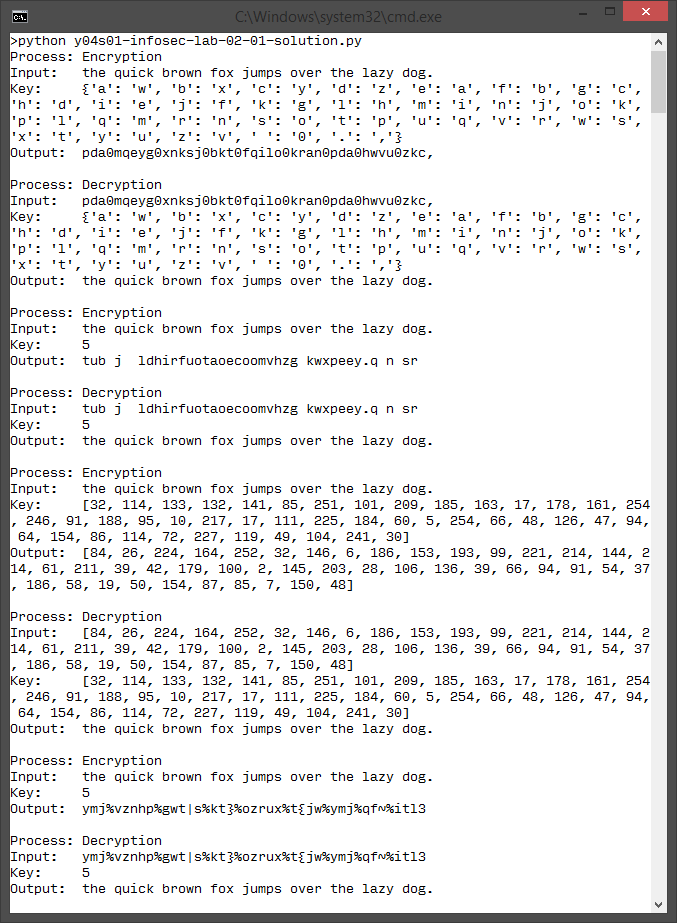
\includegraphics[height = 16\baselineskip]{./assets/00.png}
				\caption{Результат шифрування повідомлення розробленим програмним модулем}
				\label{fig:script-encryption-res}
			\end{figure}

			Бачимо, що розроблені реалізації дійсно шифрують задане повідомлення і вірно розшифровують його, тому необхідні алгоритми шифрування різних категорій були правильно реалізовані.

		\subsection{Знайомство із засобами командного рядка~\textenglish{Windows} для хешування}
			Завдання лабораторної роботи вимагає ознайомитись із програмами для операційної системи~\textenglish{Windows}, призначеними для обчислення хеш-сум за допомогою командного рядка, а саме~\textenglish{HashConsole}, \textenglish{HashUtils} і \textenglish{rhash}.

			Щоб ознайомитись із програмами, спробуємо обчислити хеш-суму певного файлу. Для цього запускаємо програми із необхідними параметрами і бачимо результат~(рис.~\ref{fig:win-cmd-hash-results}).

			\begin{figure}[!htbp]
				\begin{subfigure}[b]{6\gridunitwidth - 1em / 2}
					\centering
					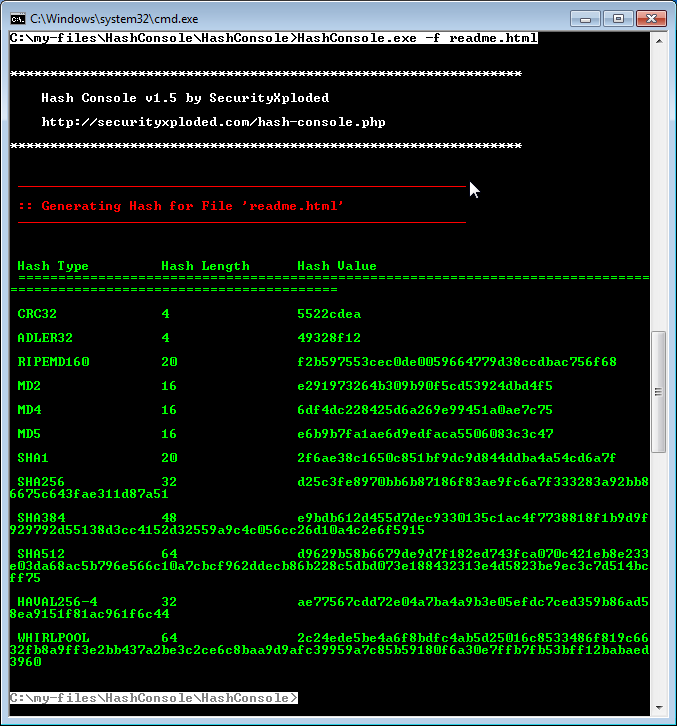
\includegraphics[width = \columnwidth]{./assets/01.png}
					\caption{}
					\label{subfig:win-cmd-hash-results-hashconsole}
				\end{subfigure}%
				\hspace{1em}
				\begin{subfigure}[b]{6\gridunitwidth - 1em / 2}
					\centering
					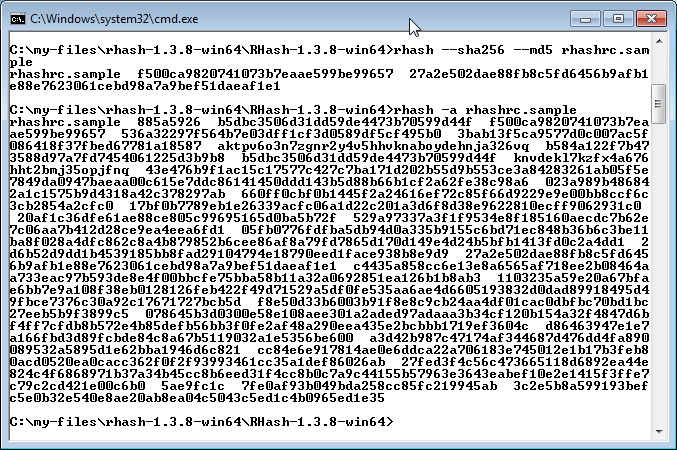
\includegraphics[width = \columnwidth]{./assets/02.png}
					\caption{}
					\label{subfig:win-cmd-hash-results-rhash}
				\end{subfigure}
				\begin{subfigure}{6\gridunitwidth - 1em / 2}
					\centering
					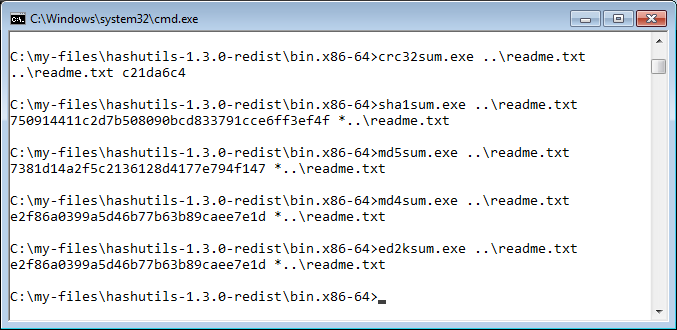
\includegraphics[width = \columnwidth]{./assets/04.png}
					\caption{}
					\label{subfig:win-cmd-hash-results-hashutils}
				\end{subfigure}%
				\caption{Результат обчислення хеш-сум файлів за допомогою запропонованих програм: \subref{subfig:win-cmd-hash-results-hashconsole}~— \textenglish{HashConsole}, \subref{subfig:win-cmd-hash-results-rhash}~— \textenglish{RHash}, \subref{subfig:win-cmd-hash-results-hashutils}~— \textenglish{hashutils}}
				\label{fig:win-cmd-hash-results}
			\end{figure}

			Усі програми дали очікуваний результат, тому ми переконались, що вони вірно встановлені і справно працюють.

		\subsection{Знайомство з графічними засобами перевірки хеш-сум}
			Для обчислення та перевірки хеш-суми за допомогою графічного інтерфейсу, використаємо відповідну можливість програми-архіватора~\textenglish{7-Zip}. Відкриваємо Провідник, виділяємо файл, хеш-суму якого необхідно обчислити, відриваємо контекстне меню, натиснувши праву клавішу миші, та обираємо пункт~\menu{CRC SHA > *}, щоб обчислити хеш-суми файлу за допомогою усіх доступних алгоритмів. В результаті бачимо обчислені хеш-суми~(рис.~\ref{fig:7zip-hashes}).

			\begin{figure}[!htbp]
				\centering
				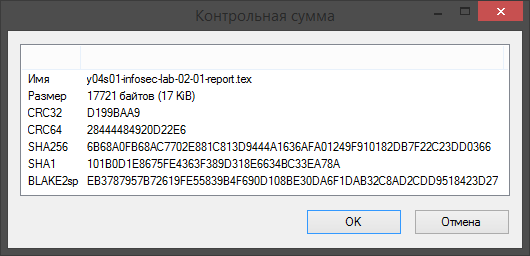
\includegraphics[height = 8 \baselineskip]{./assets/05.png}
				\caption{Результат обчислення хеш-сум за допомогою програми~\textenglish{7-Zip}}
				\label{fig:7zip-hashes}
			\end{figure}

			Як бачимо, незважаючи на те, що обчислення хеш-сум не є основним призначенням архіватора~\textenglish{7-Zip}, він все одно надає цю можливість.

		\subsection{Знайомство із засобами обчислення хеш-сум командного рядка~\textenglish{\allcaps{GNU}/Linux}}
			В операційній системі~\textenglish{\allcaps{GNU}/Linux} за замовчуванням встановлені інструменти для обчислення хеш-сум, зокрема~\progname{md5sum}, \progname{sha1sum} та \progname{sha256sum}. Використаємо їх для обчислення хеш-сум певного файлу. Для цього запускаємо їх, вказуємо ім'я бажаного файла як параметр і бачимо результат~(рис.~\ref{fig:linux-hash}).

			\begin{figure}[!htbp]
				\centering
				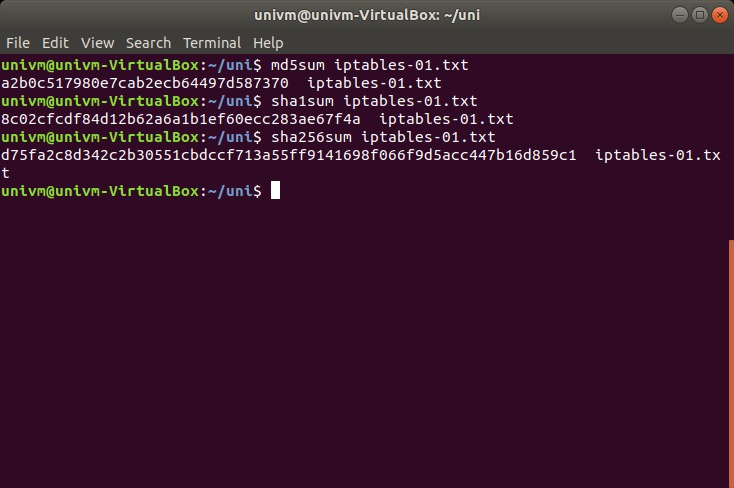
\includegraphics[height = 12 \baselineskip]{./assets/06.jpeg}
				\caption{Обчислення хеш-суми файлу за допомогою засобів командного рядка операційної системи~\textenglish{Ubuntu}}
				\label{fig:linux-hash}
			\end{figure}

			Як бачимо, обрані засоби повернули правдоподібні значення, тому можна сказати, що вони справно працюють.

		\subsection{Знайомство з алгоритмом~\textenglish{\allcaps{MD5}}}
			Знайомимось із алгоритмом~\textenglish{\allcaps{MD5}}. Це алгоритм обчислення хеш-суми, побудований на основі структури Меркла—Дамгора, складається з 4 раундів обчислення і повертає 128-бітне значення. У 2013 році дослідники представили атаку, яка зламує стійкість алгоритму~\textenglish{\allcaps{MD5}} до колізій за~$2^{18}$ часу.

			Щоб перевірити коректність реалізації алгоритму~\textenglish{\allcaps{MD5}}, обчислимо хеш-суми еталонних повідомлень: пустого символьного рядка «» та фрази «\textenglish{The quick brown fox jumps over the lazy dog}»~(рис.~\ref{fig:md5-reference}).

			\begin{figure}[!htbp]
				\centering
				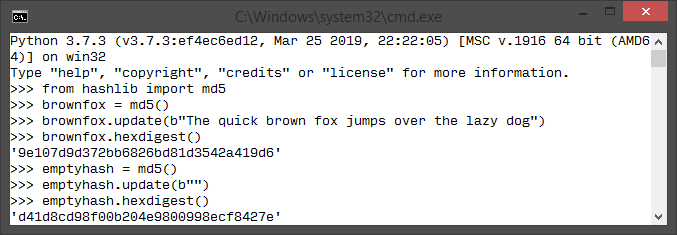
\includegraphics[height = 8 \baselineskip]{./assets/07.png}
				\caption{Обчислення хеш-сум еталонних повідомлень}
				\label{fig:md5-reference}
			\end{figure}

			Значення хеш-сум обох вхідних рядків співпадають з еталонними, отже можна стверджувати, що алгоритм~\textenglish{\allcaps{MD5}} реалізований правильно.

	\section{Висновок}
		Виконуючи дану лабораторну роботу, ми ознайомились з~основними поняттями криптографії, а також поняттями дайджеста повідомлення та деякими засобами його отримання та перевірки.

	\appendix
	\section{Початковий код програмної реалізації модуля шифрування}
	\label{sec:script-encryption-source-code}
	\inputpython{../01-solution/y04s01-infosec-lab-02-01-solution.py}{Початковий код~програмного модуля для шифрування повідомлення}{lst:encryption-script}

\end{document}
